\section{Multisalt experiments}
\prettyinpink{Generelt: Der er både tendenser i løbet af en filtrering og over varierende pH fortæl/afbild hvad der er vigtigst (hold det kort!}

The pH increased slightly in each experiment \prettyinpink{er plot nødvendigt?}
9.31 -> 9.44
10.08 -> 10.24 (shorter experiment)
10.47 -> 10.59
HCl content was not measured \prettyinpink{kan vi undvære at nævne det?}
Water mystery (will not be mentioned)
Pressure increased during filtration for all experiments, likely a result of osmotic pressure.
pH 10 experiment was shorter \prettyinpink{for reasons?}


\subsection{Bicarbonate}

The complex ion solutions were analysed for their bicarbonate content by measuring total alkalinity \rod{Tjek op på dette!}.
Samples were taken from the feed container in each experiment at various times during the filtrations and are plotted on \Cref{fig:bicarbonate_multi_salt}.

For the solutions with pH 10 and 10.5 bicarbonate content is initially ~380 \si{\milli\gram\per\liter} whereas the pH 9.2 solution initially has a slightly greater concentration at 465 \si{\milli\gram\per\liter}
It is generally observed that bicarbonate concentration increases as filtration progresses at all pH values.
For pH 9.2 and pH 10 the bicarbonate content increases to 998 and 963 \si{\milli\gram\per\liter} bicarbonate, respectively.
The bicarbonate concentration for the matrix with a pH of 10.5 initially doesn't increase during the first six hours.
The final value, however, was 1220 \si{\milli\gram\per\liter} which is the maximum possible value for the alkalinity analysis.

This large increase in measured bicarbonate may be a result of increasing silica concentrations as it was speculated was the case in the binary ion experiment \rod{måsk en ref}.

\begin{figure}[H]
    \centering
    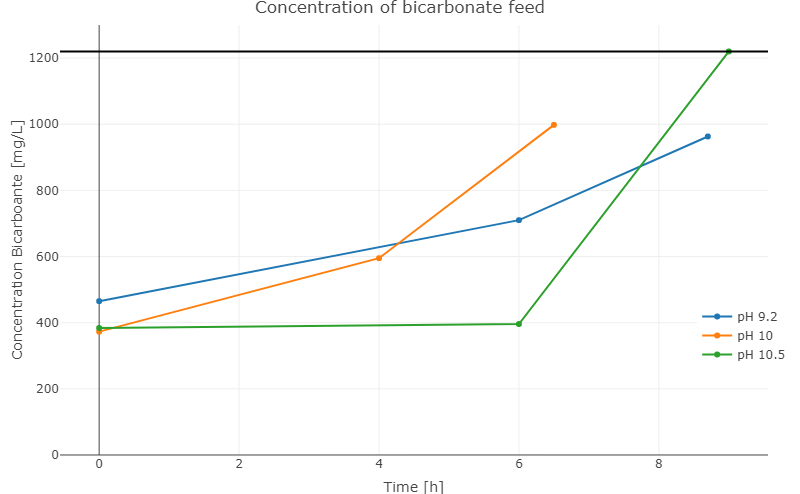
\includegraphics[width=0.8\textwidth]{Billeder/data/multi_salt/bicarbonate_all_pH.png}
    \caption{Bicarbonate concentration as determined by alkalinity}
    \label{fig:bicarbonate_multi_salt}
\end{figure}

\subsection{Silica}
Analysed by Hach Lange kits as in binary experiment \rod{stats}

The silica rejection increases with pH of the solution.
It is likely a result of increased charge density at higher pH values, which is more easily retained by the negative membrane surface(which may also be affected by solution pH).
At all pH values silica rejection increases as filtration progresses.
pH increases slightly during the filtration (which in turn may be caused by increased silica concentration) and may be the cause of the increasing rejection during a filtration at least in part. 

The dip for pH 9.2 is weird
Numbers:
pH 9.2: 21.2 ->27.4 with a dip to 8.8
pH 10: 49.5 ->58.7
pH 10.5: 65 ->72.7 (and final measurement dips to 71.3)

The measured bicarbonate by alkalinity is likely not independent from the concentration of silica.
In order to better understand how these correlate alkalinity/bicarbonate concentration has been plotted as a function of silica concentration in \Cref{fig:multi_salt_bicarbonate_+_silica_less_ugly}.
For the two lowest pH values there is a linear relationship between silica content and measured bicarbonate.
The data for pH 10.5 shows deviation with its second data point which has and increase of XX silica without any correlating increase in measure bicarbonate.
Ignoring this data point the correlation would follow that of pH 10.

\begin{figure}[H]
    \centering
    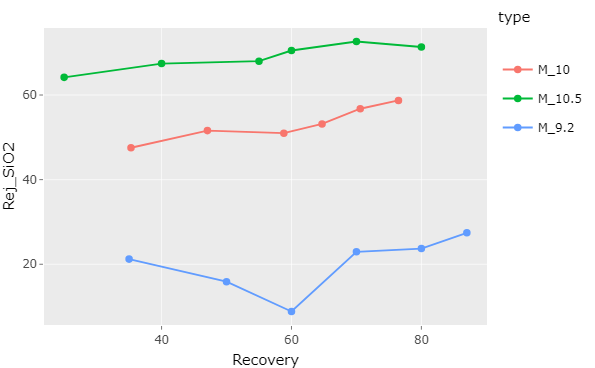
\includegraphics[width=0.8\textwidth]{Billeder/data/multi_salt/silica_rejection.png}
    \caption{Rejection of silica at different pH values}
    \label{fig:silica_rejection_multi_salt}
\end{figure}

\subsection{Bicarb + silica}
\begin{figure}[H]
    \centering
    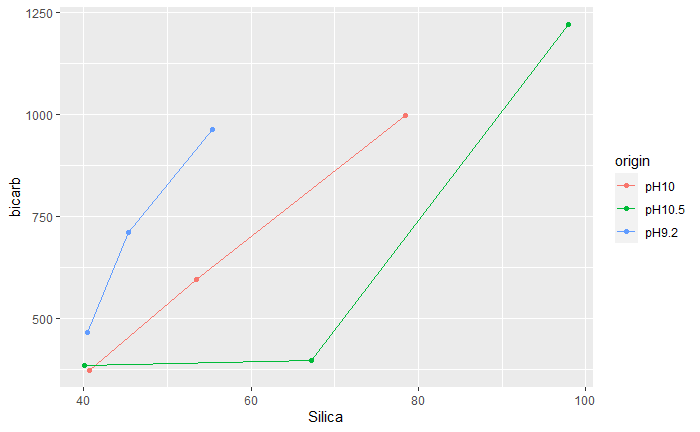
\includegraphics[width=0.8\textwidth]{Billeder/data/multi_salt/silica_bicarb_individual.png}
    \caption{Bicarbonate concentration correlates with silica concentration}
    \label{fig:multi_salt_bicarbonate_silica_releation_individual}
\end{figure}

\begin{figure}[H]
    \centering
    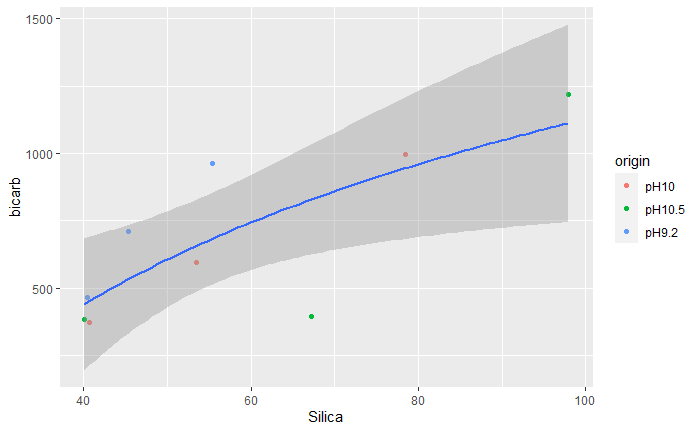
\includegraphics[width=0.8\textwidth]{Billeder/data/multi_salt/silica_bicarb_samlet.png}
    \caption{Jeg håber det er et mindre klamt plot til at se hvordan silica og bicarbonat hænger sammen, om det giver mere mening ved jeg ikke}
    \label{fig:multi_salt_bicarbonate_+_silica_less_ugly}
\end{figure}

% \begin{figure}[H]
%     \centering
%     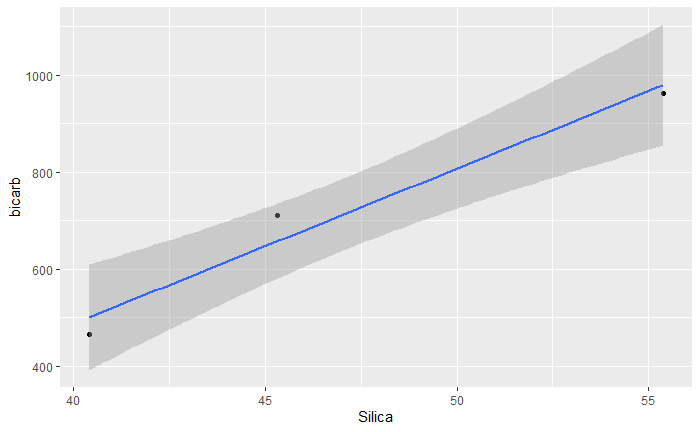
\includegraphics[width=0.8\textwidth]{Billeder/data/multi_salt/pH_9.2_silica_bicarb.png}
%     \caption{Her kun for enkelt pH (9.2)}
%     \label{fig:multi_salt_pH_9.2_bicarbonate_+_silica}
% \end{figure}
 Individuelt er der linær relation mellem silica indhold og målt bicarb

% ¤¤¤ION REJECTIONS FOR EXPERIMENTS INDIVIDUALLY¤¤¤
% \begin{figure}[H]
%     \centering
%     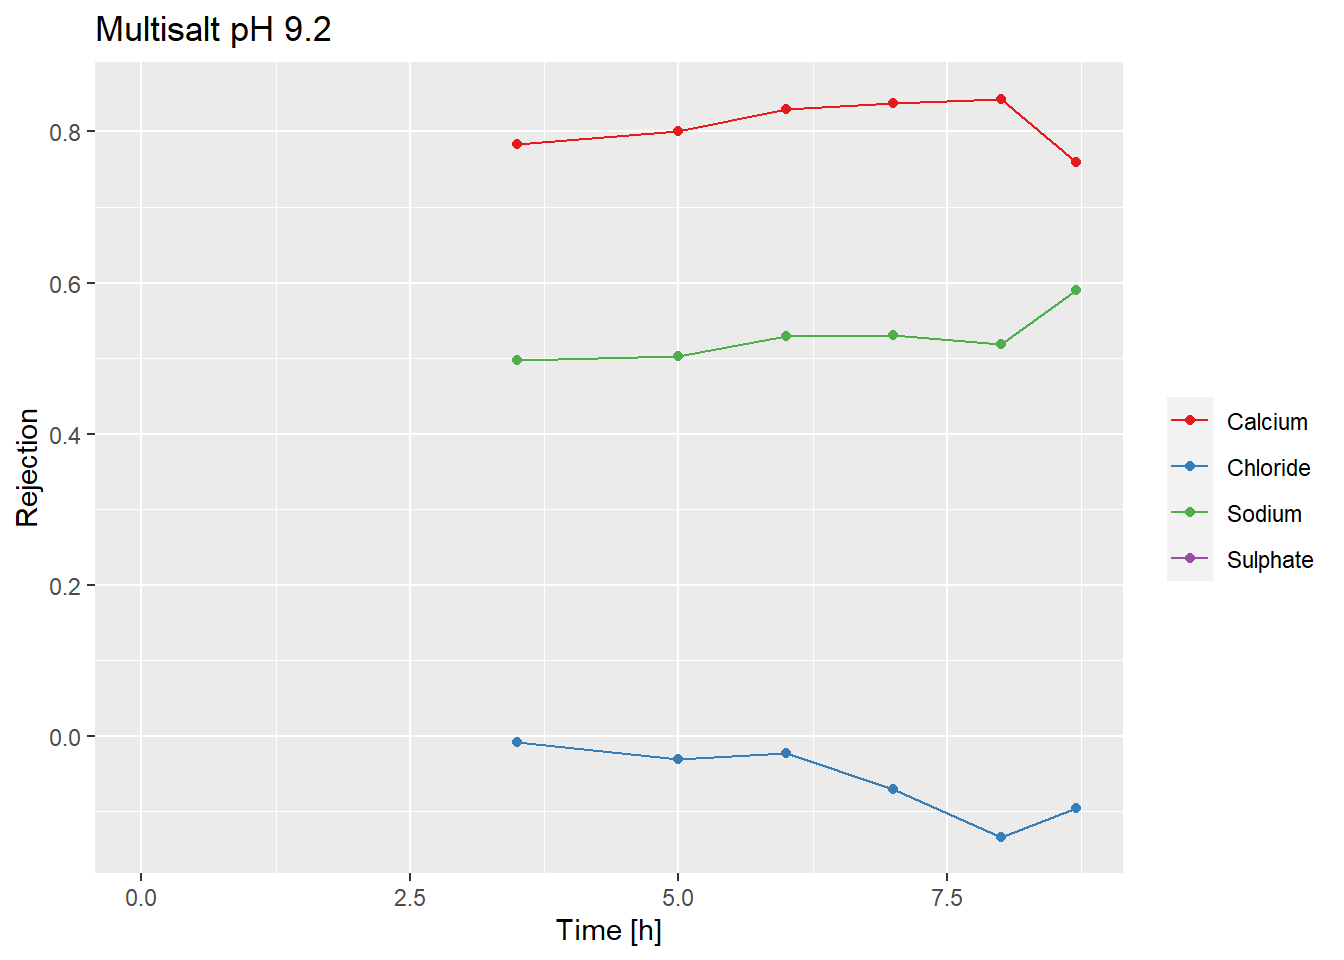
\includegraphics[width=0.8\textwidth]{Billeder/data/multi_salt/pH_9.2_ion_rejection.png}
%     \caption{Rejection during experiment with pH = 9.2}
%     \label{fig:multi_salt_pH_9.2_ion_rejection}
% \end{figure}


% \begin{figure}[H]
%     \centering
%     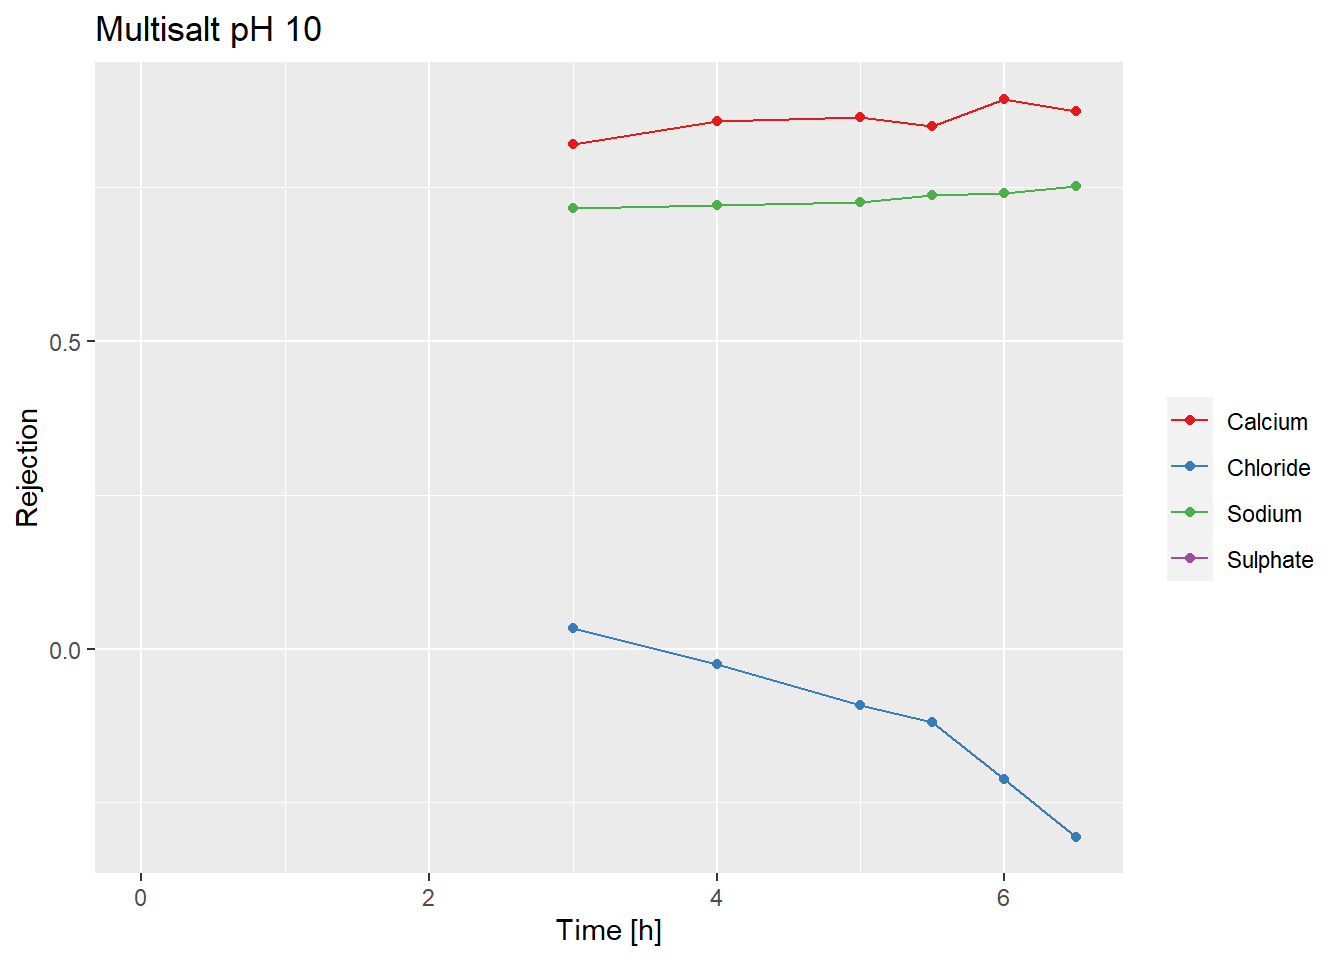
\includegraphics[width=0.8\textwidth]{Billeder/data/multi_salt/pH_10_ion_rejection.png}
%     \caption{Rejection during experiment with pH = 10}
%     \label{fig:multi_salt_pH_10_ion_rejection}
% \end{figure}


% \begin{figure}[H]
%     \centering
%     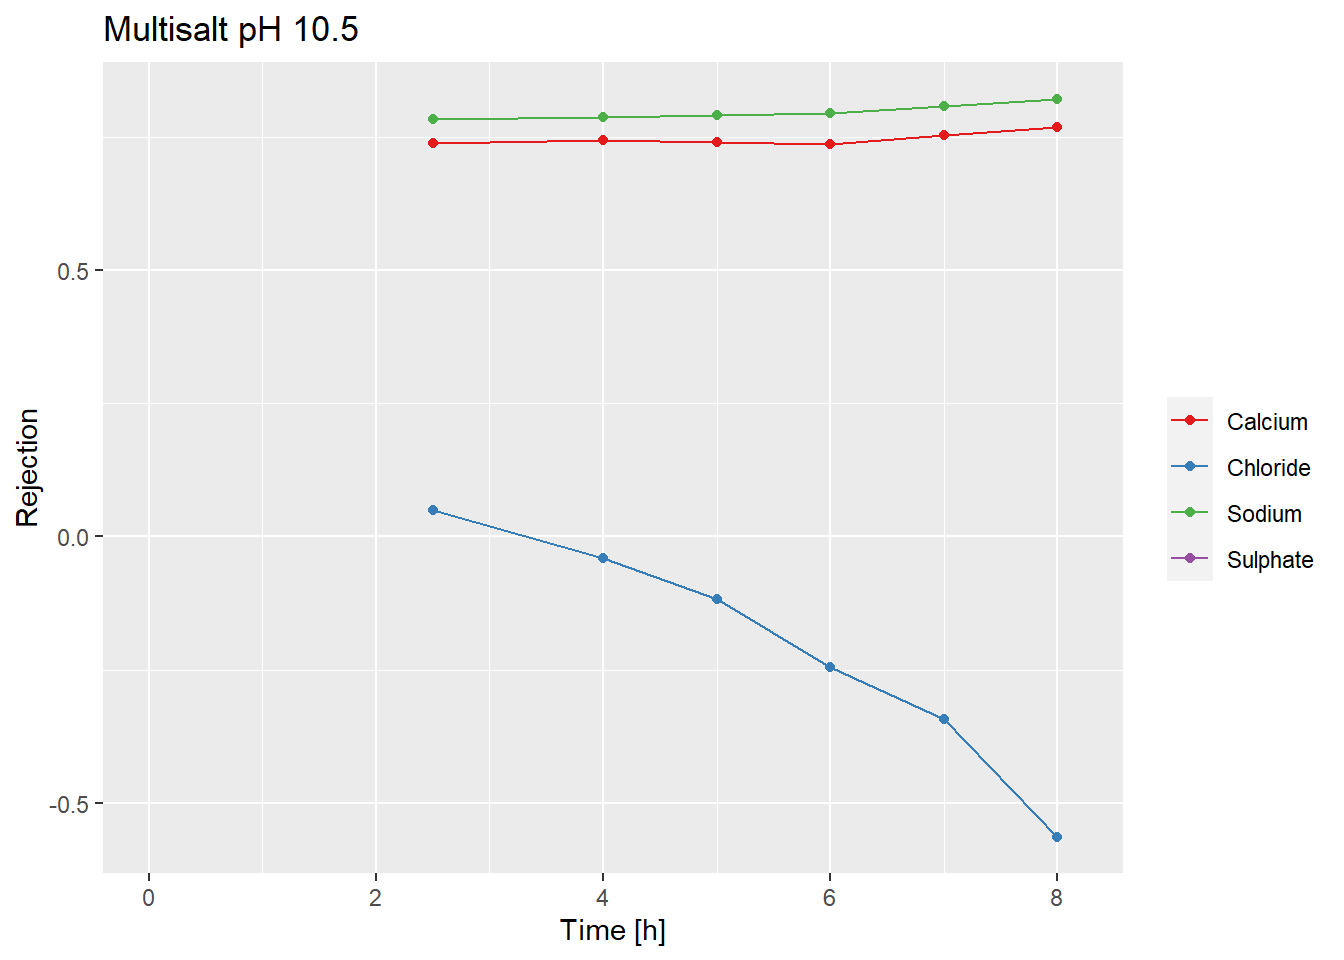
\includegraphics[width=0.8\textwidth]{Billeder/data/multi_salt/pH_10.5_ion_rejection.png}
%     \caption{Rejection during experiment with pH = 10.5}
%     \label{fig:multi_salt_pH_10.5_ion_rejection}
% \end{figure}
% ¤¤¤                                              ¤¤¤
\subsection{Ionic Rejection}
Samples were taken from feed tank and permeate and analysed by IC similar to in the binary ion experiment \rod{stats + ref}
The progression of ion rejection at each pH value plotted on \Cref{fig:multi_salt_pH_ion_rejections_samlet_med_sulfat_og_silica} along with the silica rejection.

The sulphate concentrations of the permeate samples did not exceed the LOD of 5 mg/L and this value will be used to estimate rejections.
Assuming permeate concentrations of 5 mg/L as a worst possible case sulphate rejection goes from 95 to 98 percent during filtration at all pH values


\begin{figure}[H]
    \centering
    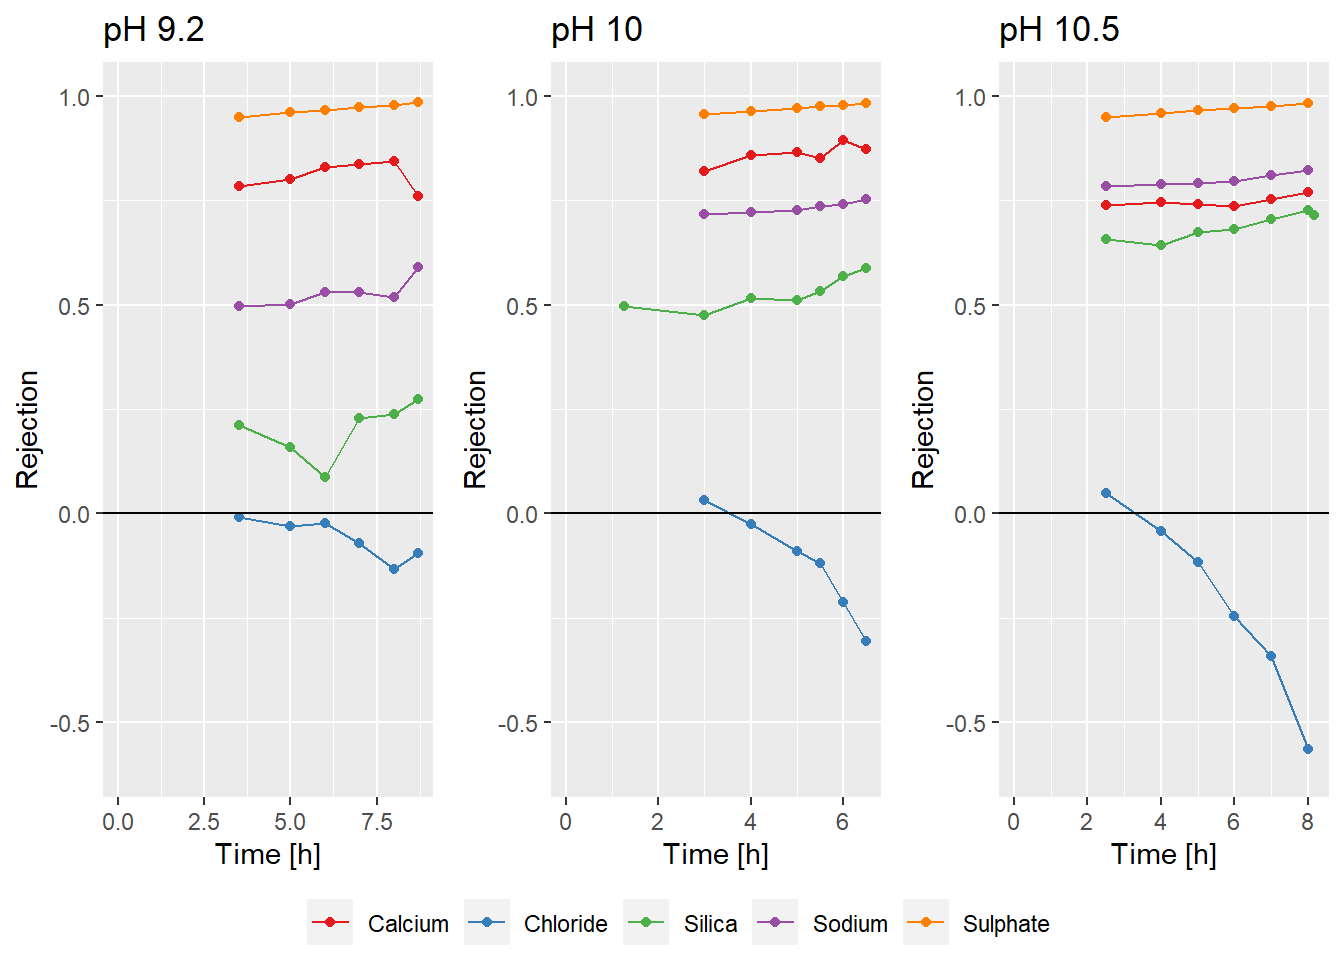
\includegraphics[width=0.8\textwidth]{Billeder/data/multi_salt/multisalt_ion_rejections_with_sulphate_and_silica.png}
    \caption{Ion Rejections for all complex ion filtrations, with sulphate rejection assuming [SO4] = 5 mg/L for permeate at all times.}
    \label{fig:multi_salt_pH_ion_rejections_samlet_med_sulfat_og_silica}
\end{figure}


\subsubsection{Overview:}
\prettyinpink{Den sidste måling for pH 9.2 er lidt weird da alle ionerne afviger fra deres ellers fine tendenser}
\textbf{Chloride:}
Chloride rejection decreases as filtration progresses for all matrix pH.

for pH 9.2 the initial rejection is just below 0 and it obtains its lowest value after 8 hours where it reaches -0.1.
for pH 10 the first measured value is just above 0 at 0.03 and declines to its final value of -0.3 after 6.5 hours.
for pH 10.5 the first measured rejection was 0.05 and this decreased to -0.56 after 8 hours.

% pH 9.2: -0.007 ->-0.096
% pH 10: 0.03 ->-0.3
% pH 10.5: 0.05 ->-0.56

It is clearly evident that chloride rejection decreases dramatically with increased pH for the values later on during the filtrations. 
\prettyinpink{træls med ingen rigtig måling af sulfat, da det burde påvirke Cl rejection, sammenlign med feed concentration}



For all pH values rejection of the other ions(i.e. not Cl-) increases slightly as each filtration progresses

\textbf{Sodium:}
Sodium rejection increases with higher pH
At pH 10.5 there is greater Na rejection than Ca rejection unlike at the other two pH levels.

Feed concentrations:
344->626
361 -> 808
404 -> 1145
\textbf{Sulphate:}
The sulphate rejection based on constant permeate concentration is 95-98\% during each filtration and is unaffected by pH change.

Feed Sulphate concentrations:
pH 9.2: 98 -> 311
pH 10: 71-> 274
pH 10.5: 69 -> 291
based on concentration profile pH 10.5 has the largest increase in sulphate concentration during the filtration, but pH 9.2 reaches highest final concentration. 


\textbf{Calcium: }
\prettyinpink{I am confusion}
Rejection is similar between pH 9.2 and 10 but lower for 10.5 where it is lower than sodium rejection
Concentrations are much higher for pH 9.2 than the other two experiments.
Feed Ca concentrations:
pH 9.2: 24 -> 46 -> 30
pH 10: 3.2 -> 19
pH 10.5: 3.6 -> 7.8




% \begin{figure}[H]
%     \centering
%     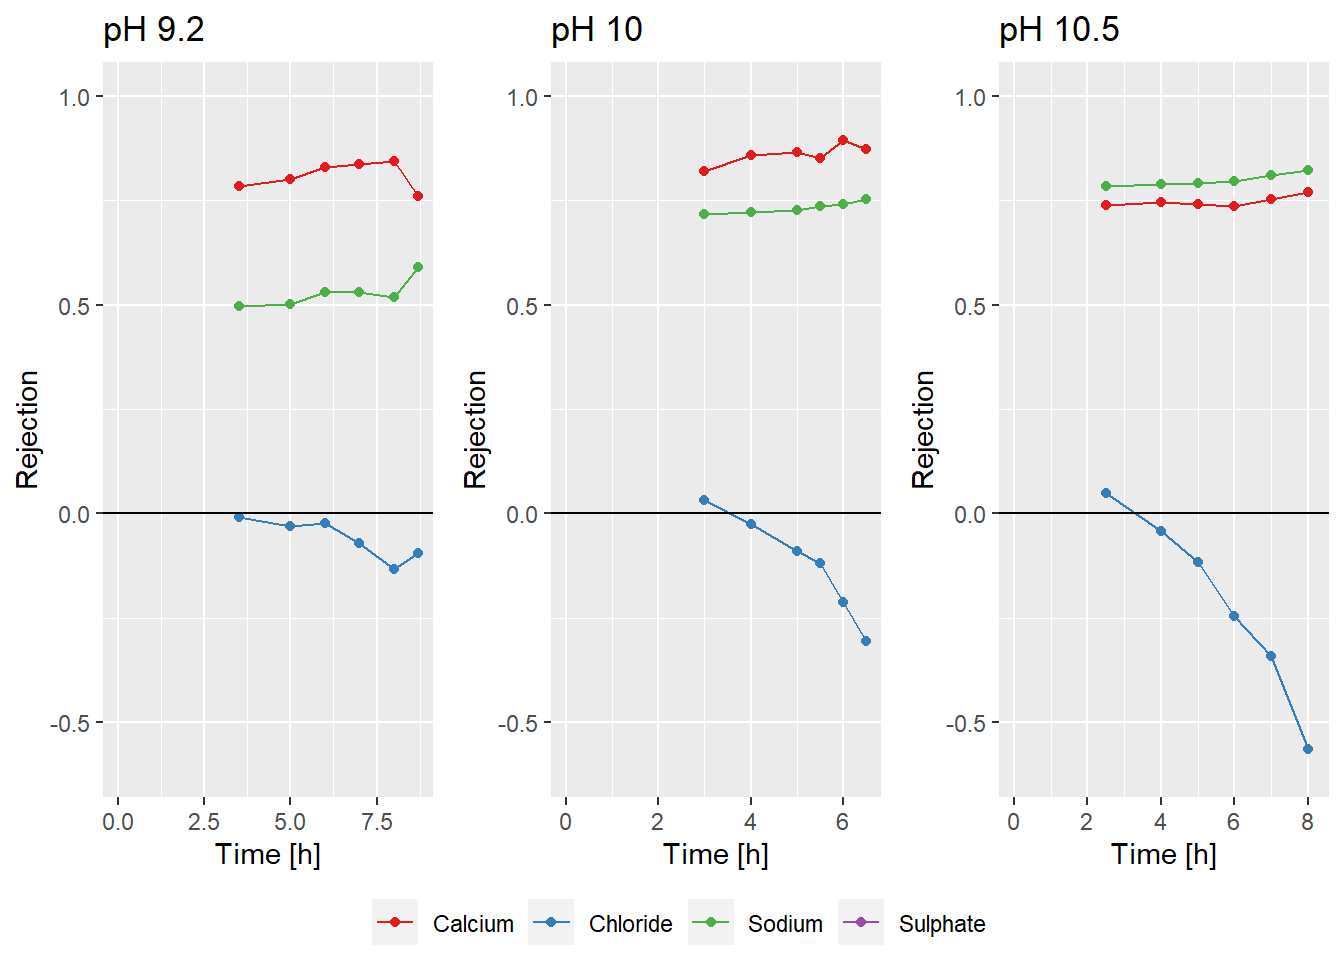
\includegraphics[width=0.8\textwidth]{Billeder/data/multi_salt/multisalt_ion_rejections.png}
%     \caption{Ion Rejections for all multisalt experiments}
%     \label{fig:multi_salt_pH_ion_rejections_samlet}
% \end{figure}

% \begin{figure}[H]
%     \centering
%     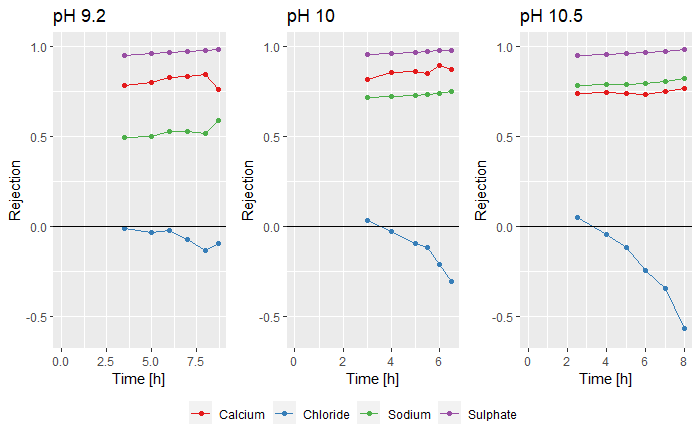
\includegraphics[width=0.8\textwidth]{Billeder/data/multi_salt/multisalt_ion_rejections_with_sulphate.png}
%     \caption{Ion Rejections for all multisalt experiments, now with sulphate rejection assuming [SO4] = 5 for permeate at all times}
%     \label{fig:multi_salt_pH_ion_rejections_samlet_med_sulfat}
% \end{figure}


